\documentclass[10pt]{beamer}

\usetheme{Madrid}
\usecolortheme{default}
\setbeamertemplate{navigation symbols}{}

\usepackage[utf8]{inputenc}
\usepackage[T1]{fontenc}
\usepackage{graphicx}
\usepackage{booktabs}
\usepackage{array}
\usepackage{adjustbox}
\usepackage{ragged2e}
\usepackage{etoolbox}
\usepackage{amsmath}
\usepackage{tikz}
\usepackage{helvet}
\renewcommand{\familydefault}{\sfdefault}
\usetikzlibrary{positioning,arrows.meta,shapes.geometric,
                shadows,backgrounds,calc,fit}
\usepackage{pgfplots}
\pgfplotsset{compat=1.18}

\definecolor{titleblue}{RGB}{26,86,159}
\definecolor{softgreen}{RGB}{0,128,80}
\definecolor{softgray}{RGB}{70,70,70}

\addtobeamertemplate{frametitle}{}{\justifying}
% Custom footer with centered text
\setbeamertemplate{footline}{%
  \begin{beamercolorbox}[wd=\paperwidth,ht=3ex,dp=1ex]{author in head/foot}
    \usebeamercolor[fg]{author in head/foot}
    \hspace{0.3cm}
    \insertframenumber{} / 26
    \hfill
    Indian Institute of Information Technology Kottayam
    \hfill
    \hspace{0.3cm}
  \end{beamercolorbox}
}

% --- REPLACE YOUR CURRENT FRAMETITLE TEMPLATE WITH THIS ---
\setbeamertemplate{frametitle}{
  \nointerlineskip
  \begin{beamercolorbox}[wd=\paperwidth,ht=1.1cm,dp=0.35cm]{frametitle}
    \hspace{0.3cm}%
    \parbox[c]{0.75\textwidth}{\usebeamerfont{frametitle}\insertframetitle}%
    \hfill%
    \parbox[c]{0.15\textwidth}{\raggedleft
\includegraphics[height=0.85cm]{logo.jpg}}%
    \hspace{0.3cm}
  \end{beamercolorbox}
}

\newcommand{\ArchitectureDiagram}[1]{%
\resizebox{#1\textwidth}{!}{%
\begin{tikzpicture}[
    node distance=1.5cm and 1cm,
    % FIXED: Changed #1 to ##1 to prevent macro argument clashing
    layerBox/.style={rectangle, draw=##1!80, fill=##1!10, dashed, thick, rounded corners=15pt, inner sep=15pt},
    appNode/.style={rectangle, draw=cyan!80!blue, fill=cyan!15, rounded corners=5pt, minimum width=3cm, minimum height=1.2cm, align=center, font=\small\bfseries, text=black!80},
    apiNode/.style={rectangle, draw=orange!80!red, fill=orange!15, rounded corners=5pt, minimum width=4cm, minimum height=1.2cm, align=center, font=\small\bfseries, text=black!80},
    scNode/.style={rectangle, draw=green!70!black, fill=green!15, rounded corners=5pt, minimum width=4cm, minimum height=1.2cm, align=center, font=\small\bfseries, text=black!80},
    storeNode/.style={rectangle, draw=purple!70, fill=purple!15, rounded corners=5pt, minimum width=4cm, minimum height=1.2cm, align=center, font=\small\bfseries, text=black!80},
    layerTitle/.style={font=\Large\bfseries, anchor=south west},
    layerSub/.style={font=\footnotesize, text=gray!80!black, anchor=north west},
    solidArrow/.style={-{Stealth[scale=1.2]}, thick, draw=gray!90!black},
    dashedArrow/.style={-{Stealth[scale=1.2]}, thick, dashed, draw=gray!90!black}
]

% ================= APPLICATION LAYER =================
\node[appNode] (doctor) {Doctor\\Dashboard};
\node[appNode, right=0.6cm of doctor] (patient) {Patient\\Dashboard};
\node[appNode, right=0.6cm of patient] (delegate) {Delegate\\View};
\node[appNode, right=0.6cm of delegate] (admin) {Admin\\Panel};

\node[layerTitle, text=cyan!80!blue] (appTitle) at ([yshift=1cm, xshift=-0.5cm]doctor.north west) {Application Layer};
\node[layerSub] (appSub) at ([yshift=-0.1cm]appTitle.south west) {React, Vite, Tailwind CSS, MetaMask (Wallet)};

\begin{scope}[on background layer]
    \node[layerBox=cyan, fit=(doctor) (patient) (delegate) (admin) (appTitle) (appSub)] (appLayer) {};
\end{scope}

% ================= BACKEND LAYER =================
\node[apiNode, below=3.5cm of doctor, xshift=1.5cm] (api) {REST API\\(Express.js)};
\node[apiNode, right=1cm of api] (queue) {Request Queue\\\& Metadata};

\node[layerTitle, text=orange!80!red] (apiTitle) at ([yshift=1cm, xshift=-0.5cm]api.north west) {Backend Services Layer};
\node[layerSub] (apiSub) at ([yshift=-0.1cm]apiTitle.south west) {Node.js, Authentication, Payload Routing};

\begin{scope}[on background layer]
    \node[layerBox=orange, fit=(api) (queue) (apiTitle) (apiSub)] (apiLayer) {};
\end{scope}

% ================= SMART CONTRACT LAYER =================
\node[scNode, below=3.5cm of api] (registry) {Prescription Registry};
\node[scNode, below=3.5cm of queue] (oracle) {DoctorStatus Oracle};

\node[layerTitle, text=green!70!black] (scTitle) at ([yshift=1cm, xshift=-0.5cm]registry.north west) {Smart Contract Layer};
\node[layerSub] (scSub) at ([yshift=-0.1cm]scTitle.south west) {Polygon PoS, EVM, Solidity 0.8.23};

\begin{scope}[on background layer]
    \node[layerBox=green, fit=(registry) (oracle) (scTitle) (scSub)] (scLayer) {};
\end{scope}

% ================= STORAGE LAYER =================
\node[storeNode, right=2.5cm of queue, yshift=-0.5cm] (ipfs) {IPFS Network\\(Encrypted Bundles)};
\node[storeNode, below=1.5cm of ipfs] (pinata) {Pinata\\(Cloud Pinning)};

\node[layerTitle, text=purple!80!black] (storeTitle) at ([yshift=1cm, xshift=-0.5cm]ipfs.north west) {Storage Layer};
\node[layerSub] (storeSub) at ([yshift=-0.1cm]storeTitle.south west) {Content-Addressed Off-Chain};

\begin{scope}[on background layer]
    \node[layerBox=purple, fit=(ipfs) (pinata) (storeTitle) (storeSub)] (storeLayer) {};
\end{scope}

% ================= INTER-LAYER ARROWS =================
\draw[solidArrow] (apiLayer.north |- appLayer.south) -- node[right, font=\footnotesize, text=gray] {API calls} (apiLayer.north);
\draw[solidArrow] (scLayer.north |- apiLayer.south) -- node[right, font=\footnotesize, text=gray] {tx / view} (scLayer.north);
\draw[solidArrow] (apiLayer.east) -- node[above, font=\footnotesize, text=gray] {pin / fetch} (apiLayer.east -| storeLayer.west);
\draw[dashedArrow] (scLayer.east) -- node[above, font=\footnotesize, text=gray] {CID anchor} (scLayer.east -| storeLayer.west);
\draw[dashedArrow] (appLayer.south -| admin.south) -- node[right, font=\footnotesize, text=gray] {CID fetch} (storeLayer.north -| admin.south);

% ================= LEGEND =================
\node[anchor=west, font=\footnotesize\color{gray}] (legend1text) at ([yshift=-1.5cm, xshift=1cm]scLayer.south west) {Direct call / transaction};
\draw[solidArrow] ([xshift=-1.5cm]legend1text.west) -- ([xshift=-0.2cm]legend1text.west);

\node[anchor=west, font=\footnotesize\color{gray}] (legend2text) at ([xshift=4cm]legend1text.east) {Content addressing / browser-side};
\draw[dashedArrow] ([xshift=-1.5cm]legend2text.west) -- ([xshift=-0.2cm]legend2text.west);

\end{tikzpicture}%
}%
}

\newcommand{\WorkflowDiagram}[1]{%
\begin{tikzpicture}[font=\sffamily\scriptsize, scale=#1, every node/.style={transform shape}]
  \tikzset{
    lane/.style={rectangle, rounded corners=4pt, minimum width=2.0cm, minimum height=0.6cm, align=center, thick, draw=gray!55, fill=white, drop shadow={opacity=0.12}},
    msg/.style={-{Stealth[length=2.7mm]}, thick},
    guide/.style={dashed, draw=gray!55}
  }

  \node[lane, fill=green!10, draw=green!50] (d) at (0,0) {\textbf{Doctor}};
  \node[lane, fill=cyan!10, draw=cyan!55] (b) at (3.6,0) {\textbf{Backend/IPFS}};
  \node[lane, fill=blue!10, draw=blue!55] (p) at (7.2,0) {\textbf{Patient}};
  \node[lane, fill=purple!10, draw=purple!55] (r) at (10.8,0) {\textbf{Registry}};

  \foreach \x in {0,3.6,7.2,10.8} {
    \draw[guide] (\x,-0.35) -- (\x,-6.6);
  }

  \draw[msg, draw=green!60!black] (0,-0.9) -- node[above, align=center] {1. encrypt + sign\\ request} (3.6,-0.9);
  \draw[msg, draw=cyan!65!black] (3.6,-1.8) -- node[above] {2. request available} (7.2,-1.8);
  \draw[msg, draw=blue!65!black] (7.2,-2.7) -- node[above] {3. fetch encrypted bundle} (3.6,-2.7);
  \draw[msg, draw=blue!65!black] (7.2,-3.6) -- node[above, align=center] {4. patient signs\\ approval} (10.8,-3.6);
  \draw[msg, draw=purple!65!black] (7.2,-4.5) -- node[above, align=center] {5. \texttt{registerPrescription()}} (10.8,-4.5);
  \draw[msg, draw=purple!65!black, dashed] (10.8,-5.3) -- node[above] {6. \texttt{PrescriptionIssued}} (7.2,-5.3);
  \draw[msg, draw=blue!65!black] (7.2,-6.1) -- node[above, align=center] {7. store tx hash\\ + id} (3.6,-6.1);
\end{tikzpicture}%
}

\newcommand{\IntegrityDiagram}[1]{%
\begin{tikzpicture}[font=\sffamily, scale=#1, every node/.style={transform shape}]
  \tikzset{
    box/.style={rectangle, rounded corners=5pt, minimum width=2.6cm, minimum height=0.8cm, align=center, thick, draw=gray!55, fill=white, drop shadow={opacity=0.12}},
    flow/.style={-{Stealth[length=3mm]}, thick, draw=gray!75},
    warn/.style={rectangle, rounded corners=5pt, minimum width=2.8cm, minimum height=0.8cm, text width=2.45cm, align=center, thick, draw=red!60, fill=red!5}
  }

  \node[box, fill=green!8, draw=green!45] (record) at (0,1.8) {\textbf{Encrypted Record}};
  \node[box, fill=blue!8, draw=blue!45] (hash) at (3.3,1.8) {\textbf{Content Hash}};
  \node[box, fill=orange!8, draw=orange!50] (cid) at (6.6,1.8) {\textbf{CID}};
  \node[box, fill=purple!8, draw=purple!55] (block) at (9.9,1.8) {\textbf{Block Anchor}};

  \draw[flow] (record) -- (hash);
  \draw[flow] (hash) -- (cid);
  \draw[flow] (cid) -- (block);

  \node[warn] (tamper) at (3.3,0.1) {\textbf{Record modified}};
  \node[warn] (newhash) at (6.6,0.1) {\textbf{Hash/CID}\\\textbf{changes}};
  \node[warn] (break) at (9.9,0.1) {\textbf{Old block no}\\\textbf{longer matches}};

  \draw[flow, draw=red!70] (tamper) -- (newhash);
  \draw[flow, draw=red!70] (newhash) -- (break);

  \node[box, fill=purple!8, draw=purple!55, minimum width=3.4cm] (next) at (13.5,1.8) {\textbf{Next Block}\\ \tiny stores previousHash};
  \draw[flow] (block) -- (next);
  \node[warn, minimum width=3.4cm, text width=3.0cm] (chainbreak) at (13.5,0.1) {\textbf{Downstream}\\\textbf{validation fails}};
  \draw[flow, draw=red!70] (break) -- (chainbreak);
\end{tikzpicture}%
}


\begin{document}

% --- SLIDE 1: TITLE PAGE STYLE ---
\begin{frame}[plain]
\centering

\vfill

\begin{beamercolorbox}[sep=8pt,center,shadow=true,rounded=true]{title}
    \usebeamerfont{title}{\bfseries\Large A BLOCKCHAIN BASED\\[0.1cm] 
    DECENTRALISED HEALTH RECORD SYSTEM}
\end{beamercolorbox}

\vfill

\footnotesize
A Project Report Submitted in Partial Fulfilment\\
of the Requirements for the Degree of\\[0.2cm]
{\large\bfseries BACHELOR OF TECHNOLOGY}\\[0.1cm]
in\\
{\normalsize\bfseries COMPUTER SCIENCE AND ENGINEERING}

\vfill

{\em by}\\[0.2cm]
\small
\begin{tabular}{c}
    \textbf{Shashank Upadhyay (2022BCS0088)}\\
    \textbf{Anushila Biswas (2022BCS0069)}\\
    \textbf{Vyshnavi Reddy Battula (2022BCS0133)}\\
    \textbf{Suraj Rathor (2022BCS0051)}
\end{tabular}

\vfill


\includegraphics[width=1.3cm]{logo.jpg}

\vfill

{\em to}\\[0.1cm]
{\footnotesize\bfseries DEPARTMENT OF COMPUTER SCIENCE AND ENGINEERING}\\
{\footnotesize\bfseries INDIAN INSTITUTE OF INFORMATION TECHNOLOGY}\\
{\footnotesize\bfseries KOTTAYAM - 686635, INDIA}\\[0.2cm]
{\it April 2026}

\vfill
\end{frame}


\begin{frame}{Declaration}
\footnotesize
\noindent We, \textbf{Shashank Upadhyay (2022BCS0088), Anushila Biswas (2022BCS0069), Vyshnavi Reddy Battula (2022BCS0133), and Suraj Rathor (2022BCS0051)}, hereby declare that this work entitled \textbf{``A Blockchain-Based Decentralised Health Record System''} is an original project carried out under the supervision of \textbf{Dr.\ Anu Maria Sebastian}. It has not formed the basis for the award of any degree or diploma in this or any other institution, and all external material has been duly acknowledged.

\vspace{0.6cm}
\noindent
\begin{minipage}[t]{0.47\textwidth}
Kottayam -- 686635\\
April 2026
\end{minipage}
\hfill
\begin{minipage}[t]{0.47\textwidth}
\raggedleft
\textbf{Shashank Upadhyay (2022BCS0088)}\\
\textbf{Anushila Biswas (2022BCS0069)}\\
\textbf{Vyshnavi Reddy Battula (2022BCS0133)}\\
\textbf{Suraj Rathor (2022BCS0051)}
\end{minipage}
\end{frame}

\begin{frame}{Certificate}
\footnotesize
\noindent This is to certify that the project report entitled \textbf{``A Blockchain Based Decentralised Health Record System''} submitted by \textbf{Shashank Upadhyay (2022BCS0088), Anushila Biswas (2022BCS0069), Vyshnavi Reddy Battula (2022BCS0133), and Suraj Rathor (2022BCS0051)} to the Indian Institute of Information Technology Kottayam, in partial fulfilment of the requirements for the degree of Bachelor of Technology in Computer Science and Engineering, has been carried out under my supervision and guidance.

\vspace{0.9cm}
\noindent
\begin{minipage}[t]{0.47\textwidth}
Kottayam -- 686635\\
April 2026
\end{minipage}
\hfill
\begin{minipage}[t]{0.47\textwidth}
\raggedleft
\textbf{(Dr.\ Anu Maria Sebastian)}\\
Project Supervisor\\
Assistant Professor, Dept. of CSE\\
IIIT Kottayam
\end{minipage}
\end{frame}

\begin{frame}{Literature Survey and Identified Gap}
\footnotesize
\begin{adjustbox}{max width=\textwidth}
\begin{tabular}{@{}p{3.1cm}p{4.2cm}p{4.4cm}p{3.3cm}@{}}
\toprule
\textbf{Paper} & \textbf{What it shows} & \textbf{Useful result} & \textbf{\textcolor{red!70!black}{Gap relevant to our work}} \\
\midrule
MedRec (2016) & Early decentralized access control for health records & Auditability and blockchain feasibility & \textbf{\textcolor{red!70!black}{No protocol-level patient co-signature}} \\
\midrule
Chelladurai \& Pandian (2021) & Hyperledger Fabric EHR automation & Response time, throughput, CPU and memory evidence & \textbf{\textcolor{red!70!black}{No encrypted recipient refresh workflow}} \\
\midrule
Shuaib et al. (2022) & Besu / IBFT benchmark under load & Strongest node-load and latency style evaluation & \textbf{\textcolor{red!70!black}{No dual-signature prescription publication}} \\
\midrule
HealthChain (2024) & Secure interoperable framework & Latency / throughput / interoperability framing & \textbf{\textcolor{red!70!black}{Mostly framework-level; limited implementation detail}} \\
\bottomrule
\end{tabular}
\end{adjustbox}

\vspace{0.3cm}
\small
\textbf{Gap addressed by the proposed system:} combine patient-approved publication, oracle-based doctor authorization, encrypted off-chain storage, and reproducible evaluation in one working prototype.
\end{frame}

\begin{frame}{Why Decentralize Health Records?}
\begin{columns}[T]

\begin{column}{0.49\textwidth}
{% Group for local color change
\setbeamercolor{block title}{bg=red!70!black,fg=white}
\setbeamercolor{block body}{bg=red!10,fg=black}
\begin{block}{Centralized EHRs (Status Quo)}
\scriptsize
\begin{itemize}
    \setlength{\itemsep}{0.5ex}
    \item \textbf{Data Silos:} Isolated repositories prevent data portability and interoperability.
    \item \textbf{Single Point of Failure:} Concentrated attack surfaces invite ransomware.
    \item \textbf{Absent Patient Control:} Patients cannot practically audit or selectively share records.
\end{itemize}
\end{block}
}
\end{column}

\begin{column}{0.49\textwidth}
{% Group for local color change
\setbeamercolor{block title}{bg=blue!70!black,fg=white}
\setbeamercolor{block body}{bg=blue!10,fg=black}
\begin{block}{Blockchain EHRs (Proposed)}
\scriptsize
\begin{itemize}
    \setlength{\itemsep}{0.5ex}
    \item \textbf{Interoperable Ledger:} A shared distributed ledger eliminates isolated data silos.
    \item \textbf{Distributed Resilience:} Cryptographic chaining eliminates single points of failure.
    \item \textbf{Patient Sovereignty:} Smart contracts give programmable control over access.
\end{itemize}
\end{block}
}
\end{column}

\end{columns}

\vspace{0.1cm}
\begin{figure}
\centering
\resizebox{0.65\linewidth}{!}{
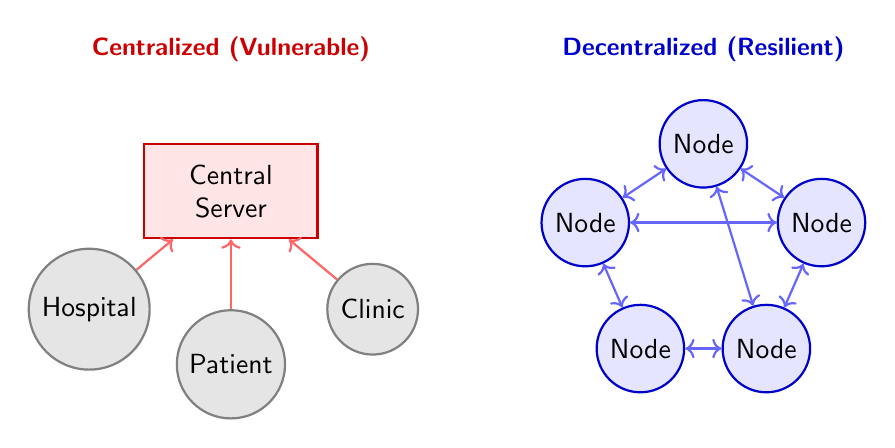
\begin{tikzpicture}[
  node distance=2cm,
  server/.style={rectangle, draw=red!80!black, fill=red!10, thick, minimum width=2.2cm, minimum height=1.2cm, align=center},
  peer/.style={circle, draw=blue!80!black, fill=blue!10, thick, minimum size=1cm, align=center},
  label/.style={font=\bfseries\small}
]

% Centralized Side
\node[label, text=red!80!black] (cent_label) at (-3, 1.8) {Centralized (Vulnerable)};
\node[server] (server) at (-3, 0) {Central\\Server};
\node[circle, draw=gray, fill=gray!20, thick] (h1) at (-4.8, -1.5) {Hospital};
\node[circle, draw=gray, fill=gray!20, thick] (h2) at (-1.2, -1.5) {Clinic};
\node[circle, draw=gray, fill=gray!20, thick] (h3) at (-3, -2.2) {Patient};

\draw[->, thick, red!60] (h1) -- (server);
\draw[->, thick, red!60] (h2) -- (server);
\draw[->, thick, red!60] (h3) -- (server);

% Decentralized Side
\node[label, text=blue!80!black] (dec_label) at (3, 1.8) {Decentralized (Resilient)};
\node[peer] (p1) at (3, 0.6) {Node};
\node[peer] (p2) at (4.5, -0.4) {Node};
\node[peer] (p3) at (3.8, -2.0) {Node};
\node[peer] (p4) at (1.5, -0.4) {Node};
\node[peer] (p5) at (2.2, -2.0) {Node};

\draw[<->, thick, blue!60] (p1) -- (p2);
\draw[<->, thick, blue!60] (p2) -- (p3);
\draw[<->, thick, blue!60] (p3) -- (p5);
\draw[<->, thick, blue!60] (p5) -- (p4);
\draw[<->, thick, blue!60] (p4) -- (p1);
\draw[<->, thick, blue!60] (p1) -- (p3);
\draw[<->, thick, blue!60] (p2) -- (p4);

\end{tikzpicture}
}
\end{figure}
\end{frame}



\begin{frame}{Definition and Scope of Work}
\small
\begin{itemize}
  \item \textbf{Problem definition:} Conventional EHR systems are siloed, institution-controlled, and difficult to audit across providers.
  \item \textbf{Goal:} Build a blockchain-based prescription record system where final publication requires both doctor intent and patient approval.
  \item \textbf{Core scope delivered:}
  \begin{itemize}
    \item off-chain encrypted storage on IPFS
    \item on-chain CID anchoring and access control
    \item doctor authorization through an oracle contract
    \item patient delegation and metadata refresh for new recipients
    \item prototype evaluation with tests, metrics, load benchmark, and simulation
  \end{itemize}
  \item \textbf{Out of scope:} production compliance certification, multi-validator deployment, hospital ERP integration, and emergency override workflow.
\end{itemize}
\end{frame}



\begin{frame}{Proposed Architecture}

\centering % Use \centering instead of \begin{center} to save vertical space
\begin{adjustbox}{max width=0.98\linewidth, max height=0.55\textheight}
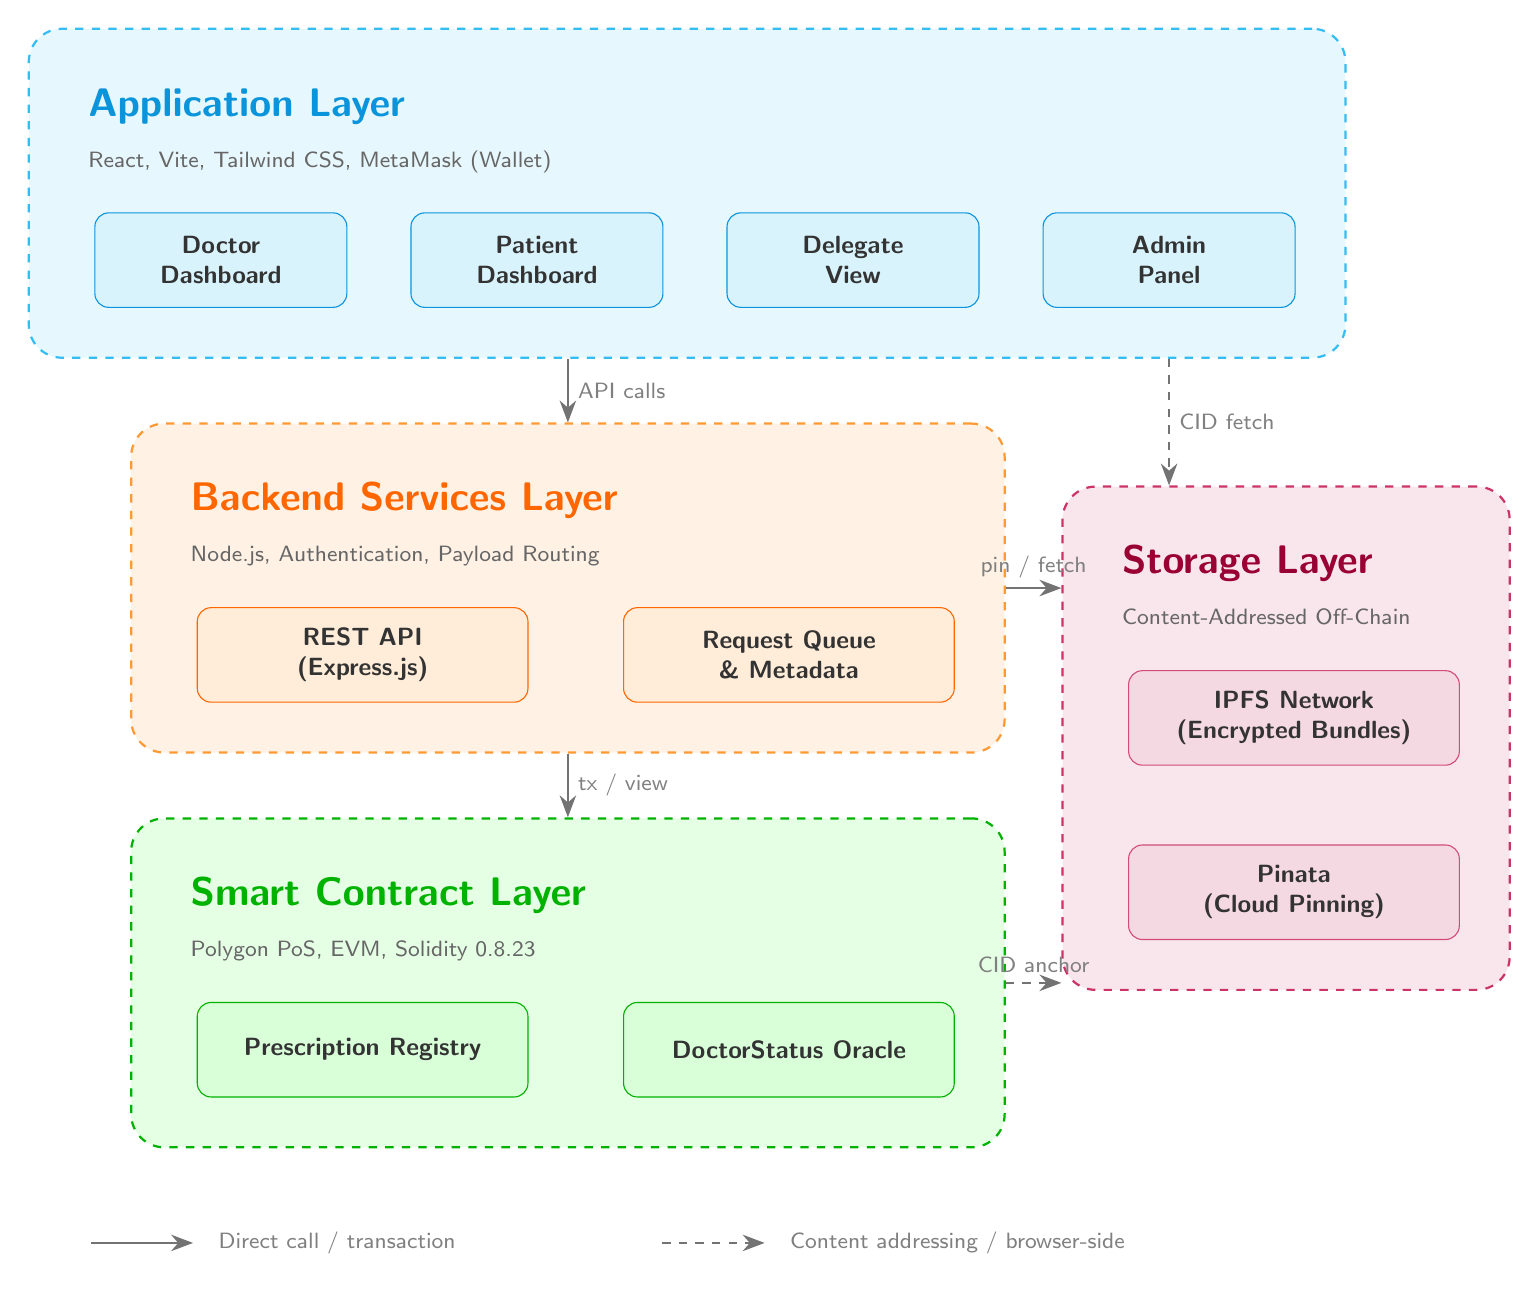
\begin{tikzpicture}[
    node distance=1.8cm and 1cm,
    layerBoxCyan/.style={rectangle, draw=cyan!80, fill=cyan!10, dashed, thick, rounded corners=12pt, inner sep=18pt},
    layerBoxOrange/.style={rectangle, draw=orange!80, fill=orange!10, dashed, thick, rounded corners=12pt, inner sep=18pt},
    layerBoxGreen/.style={rectangle, draw=green!70!black, fill=green!10, dashed, thick, rounded corners=12pt, inner sep=18pt},
    layerBoxPurple/.style={rectangle, draw=purple!80, fill=purple!10, dashed, thick, rounded corners=12pt, inner sep=18pt},
    appNode/.style={rectangle, draw=cyan!80!blue, fill=cyan!15, rounded corners=5pt, minimum width=3.2cm, minimum height=1.2cm, align=center, font=\small\bfseries, text=black!80},
    apiNode/.style={rectangle, draw=orange!80!red, fill=orange!15, rounded corners=5pt, minimum width=4.2cm, minimum height=1.2cm, align=center, font=\small\bfseries, text=black!80},
    scNode/.style={rectangle, draw=green!70!black, fill=green!15, rounded corners=5pt, minimum width=4.2cm, minimum height=1.2cm, align=center, font=\small\bfseries, text=black!80},
    storeNode/.style={rectangle, draw=purple!70, fill=purple!15, rounded corners=5pt, minimum width=4.2cm, minimum height=1.2cm, align=center, font=\small\bfseries, text=black!80},
    layerTitle/.style={font=\Large\bfseries, anchor=south west},
    layerSub/.style={font=\footnotesize, text=gray!80!black, anchor=north west},
    solidArrow/.style={-{Stealth[scale=1.2]}, thick, draw=gray!90!black},
    dashedArrow/.style={-{Stealth[scale=1.2]}, thick, dashed, draw=gray!90!black}
]

% ================= APPLICATION LAYER =================
\node[appNode] (doctor) {Doctor\\Dashboard};
\node[appNode, right=0.8cm of doctor] (patient) {Patient\\Dashboard};
\node[appNode, right=0.8cm of patient] (delegate) {Delegate\\View};
\node[appNode, right=0.8cm of delegate] (admin) {Admin\\Panel};

\node[layerTitle, text=cyan!80!blue] (appTitle) at ([yshift=1cm, xshift=-0.2cm]doctor.north west) {Application Layer};
\node[layerSub] (appSub) at ([yshift=-0.1cm]appTitle.south west) {React, Vite, Tailwind CSS, MetaMask (Wallet)};

\begin{scope}[on background layer]
    \node[layerBoxCyan, fit=(doctor) (patient) (delegate) (admin) (appTitle) (appSub)] (appLayer) {};
\end{scope}

% ================= BACKEND LAYER =================
\node[apiNode, below=3.8cm of doctor, xshift=1.8cm] (api) {REST API\\(Express.js)};
\node[apiNode, right=1.2cm of api] (queue) {Request Queue\\\& Metadata};

\node[layerTitle, text=orange!80!red] (apiTitle) at ([yshift=1cm, xshift=-0.2cm]api.north west) {Backend Services Layer};
\node[layerSub] (apiSub) at ([yshift=-0.1cm]apiTitle.south west) {Node.js, Authentication, Payload Routing};

\begin{scope}[on background layer]
    \node[layerBoxOrange, fit=(api) (queue) (apiTitle) (apiSub)] (apiLayer) {};
\end{scope}

% ================= SMART CONTRACT LAYER =================
\node[scNode, below=3.8cm of api] (registry) {Prescription Registry};
\node[scNode, below=3.8cm of queue] (oracle) {DoctorStatus Oracle};

\node[layerTitle, text=green!70!black] (scTitle) at ([yshift=1cm, xshift=-0.2cm]registry.north west) {Smart Contract Layer};
\node[layerSub] (scSub) at ([yshift=-0.1cm]scTitle.south west) {Polygon PoS, EVM, Solidity 0.8.23};

\begin{scope}[on background layer]
    \node[layerBoxGreen, fit=(registry) (oracle) (scTitle) (scSub)] (scLayer) {};
\end{scope}

% ================= STORAGE LAYER =================
\node[storeNode, right=2.2cm of queue, yshift=-0.8cm] (ipfs) {IPFS Network\\(Encrypted Bundles)};
\node[storeNode, below=1cm of ipfs] (pinata) {Pinata\\(Cloud Pinning)};

\node[layerTitle, text=purple!80!black] (storeTitle) at ([yshift=1cm, xshift=-0.2cm]ipfs.north west) {Storage Layer};
\node[layerSub] (storeSub) at ([yshift=-0.1cm]storeTitle.south west) {Content-Addressed Off-Chain};

\begin{scope}[on background layer]
    \node[layerBoxPurple, fit=(ipfs) (pinata) (storeTitle) (storeSub)] (storeLayer) {};
\end{scope}

% ================= INTER-LAYER ARROWS =================
\draw[solidArrow] (apiLayer.north |- appLayer.south) -- node[right, font=\footnotesize, text=gray] {API calls} (apiLayer.north);
\draw[solidArrow] (scLayer.north |- apiLayer.south) -- node[right, font=\footnotesize, text=gray] {tx / view} (scLayer.north);
\draw[solidArrow] (apiLayer.east) -- node[above, font=\footnotesize, text=gray] {pin / fetch} (apiLayer.east -| storeLayer.west);
\draw[dashedArrow] (scLayer.east) -- node[above, font=\footnotesize, text=gray] {CID anchor} (scLayer.east -| storeLayer.west);
\draw[dashedArrow] (appLayer.south -| admin.south) -- node[right, font=\footnotesize, text=gray] {CID fetch} (storeLayer.north -| admin.south);

% ================= LEGEND =================
\node[anchor=west, font=\footnotesize\color{gray}] (legend1text) at ([yshift=-1.2cm, xshift=1cm]scLayer.south west) {Direct call / transaction};
\draw[solidArrow] ([xshift=-1.5cm]legend1text.west) -- ([xshift=-0.2cm]legend1text.west);

\node[anchor=west, font=\footnotesize\color{gray}] (legend2text) at ([xshift=4cm]legend1text.east) {Content addressing / browser-side};
\draw[dashedArrow] ([xshift=-1.5cm]legend2text.west) -- ([xshift=-0.2cm]legend2text.west);

\end{tikzpicture}
\end{adjustbox}

\vspace{0.3cm} % Controlled spacing between diagram and text
\footnotesize % Reduced from \small to ensure it fits comfortably
\begin{itemize}
  \setlength{\itemsep}{0.5ex} % Tightened bullet spacing
  \item Browser clients handle wallet signatures and encrypted bundle preparation.
  \item Backend stores pending requests, orchestrates Pinata, and serves metadata to authorised viewers.
  \item Blockchain stores only the lightweight integrity anchor and access-control state.
\end{itemize}
\end{frame}


\begin{frame}{End-to-End Encryption \& Key Derivation}
\begin{columns}[T] 

\begin{column}{0.48\textwidth}
\footnotesize 
\begin{itemize}
  \setlength{\itemsep}{1ex} 
  \item \textbf{Data Encryption Key (DEK):} A fresh random 256-bit DEK is generated for each prescription to encrypt the payload via AES-256-GCM. 
  \item \textbf{Key Encryption Key (KEK):} Derived by hashing an EIP-712 structured-data signature produced by the recipient's MetaMask. Private keys never leave the local environment. 
  \item \textbf{Delegation Re-encryption:} During delegation, the Patient decrypts the DEK client-side and derives a new KEK for the delegate using their public address, without exposing the DEK. 
\end{itemize}
\end{column}

\begin{column}{0.52\textwidth}
\vspace{-0.8cm}
\begin{center}
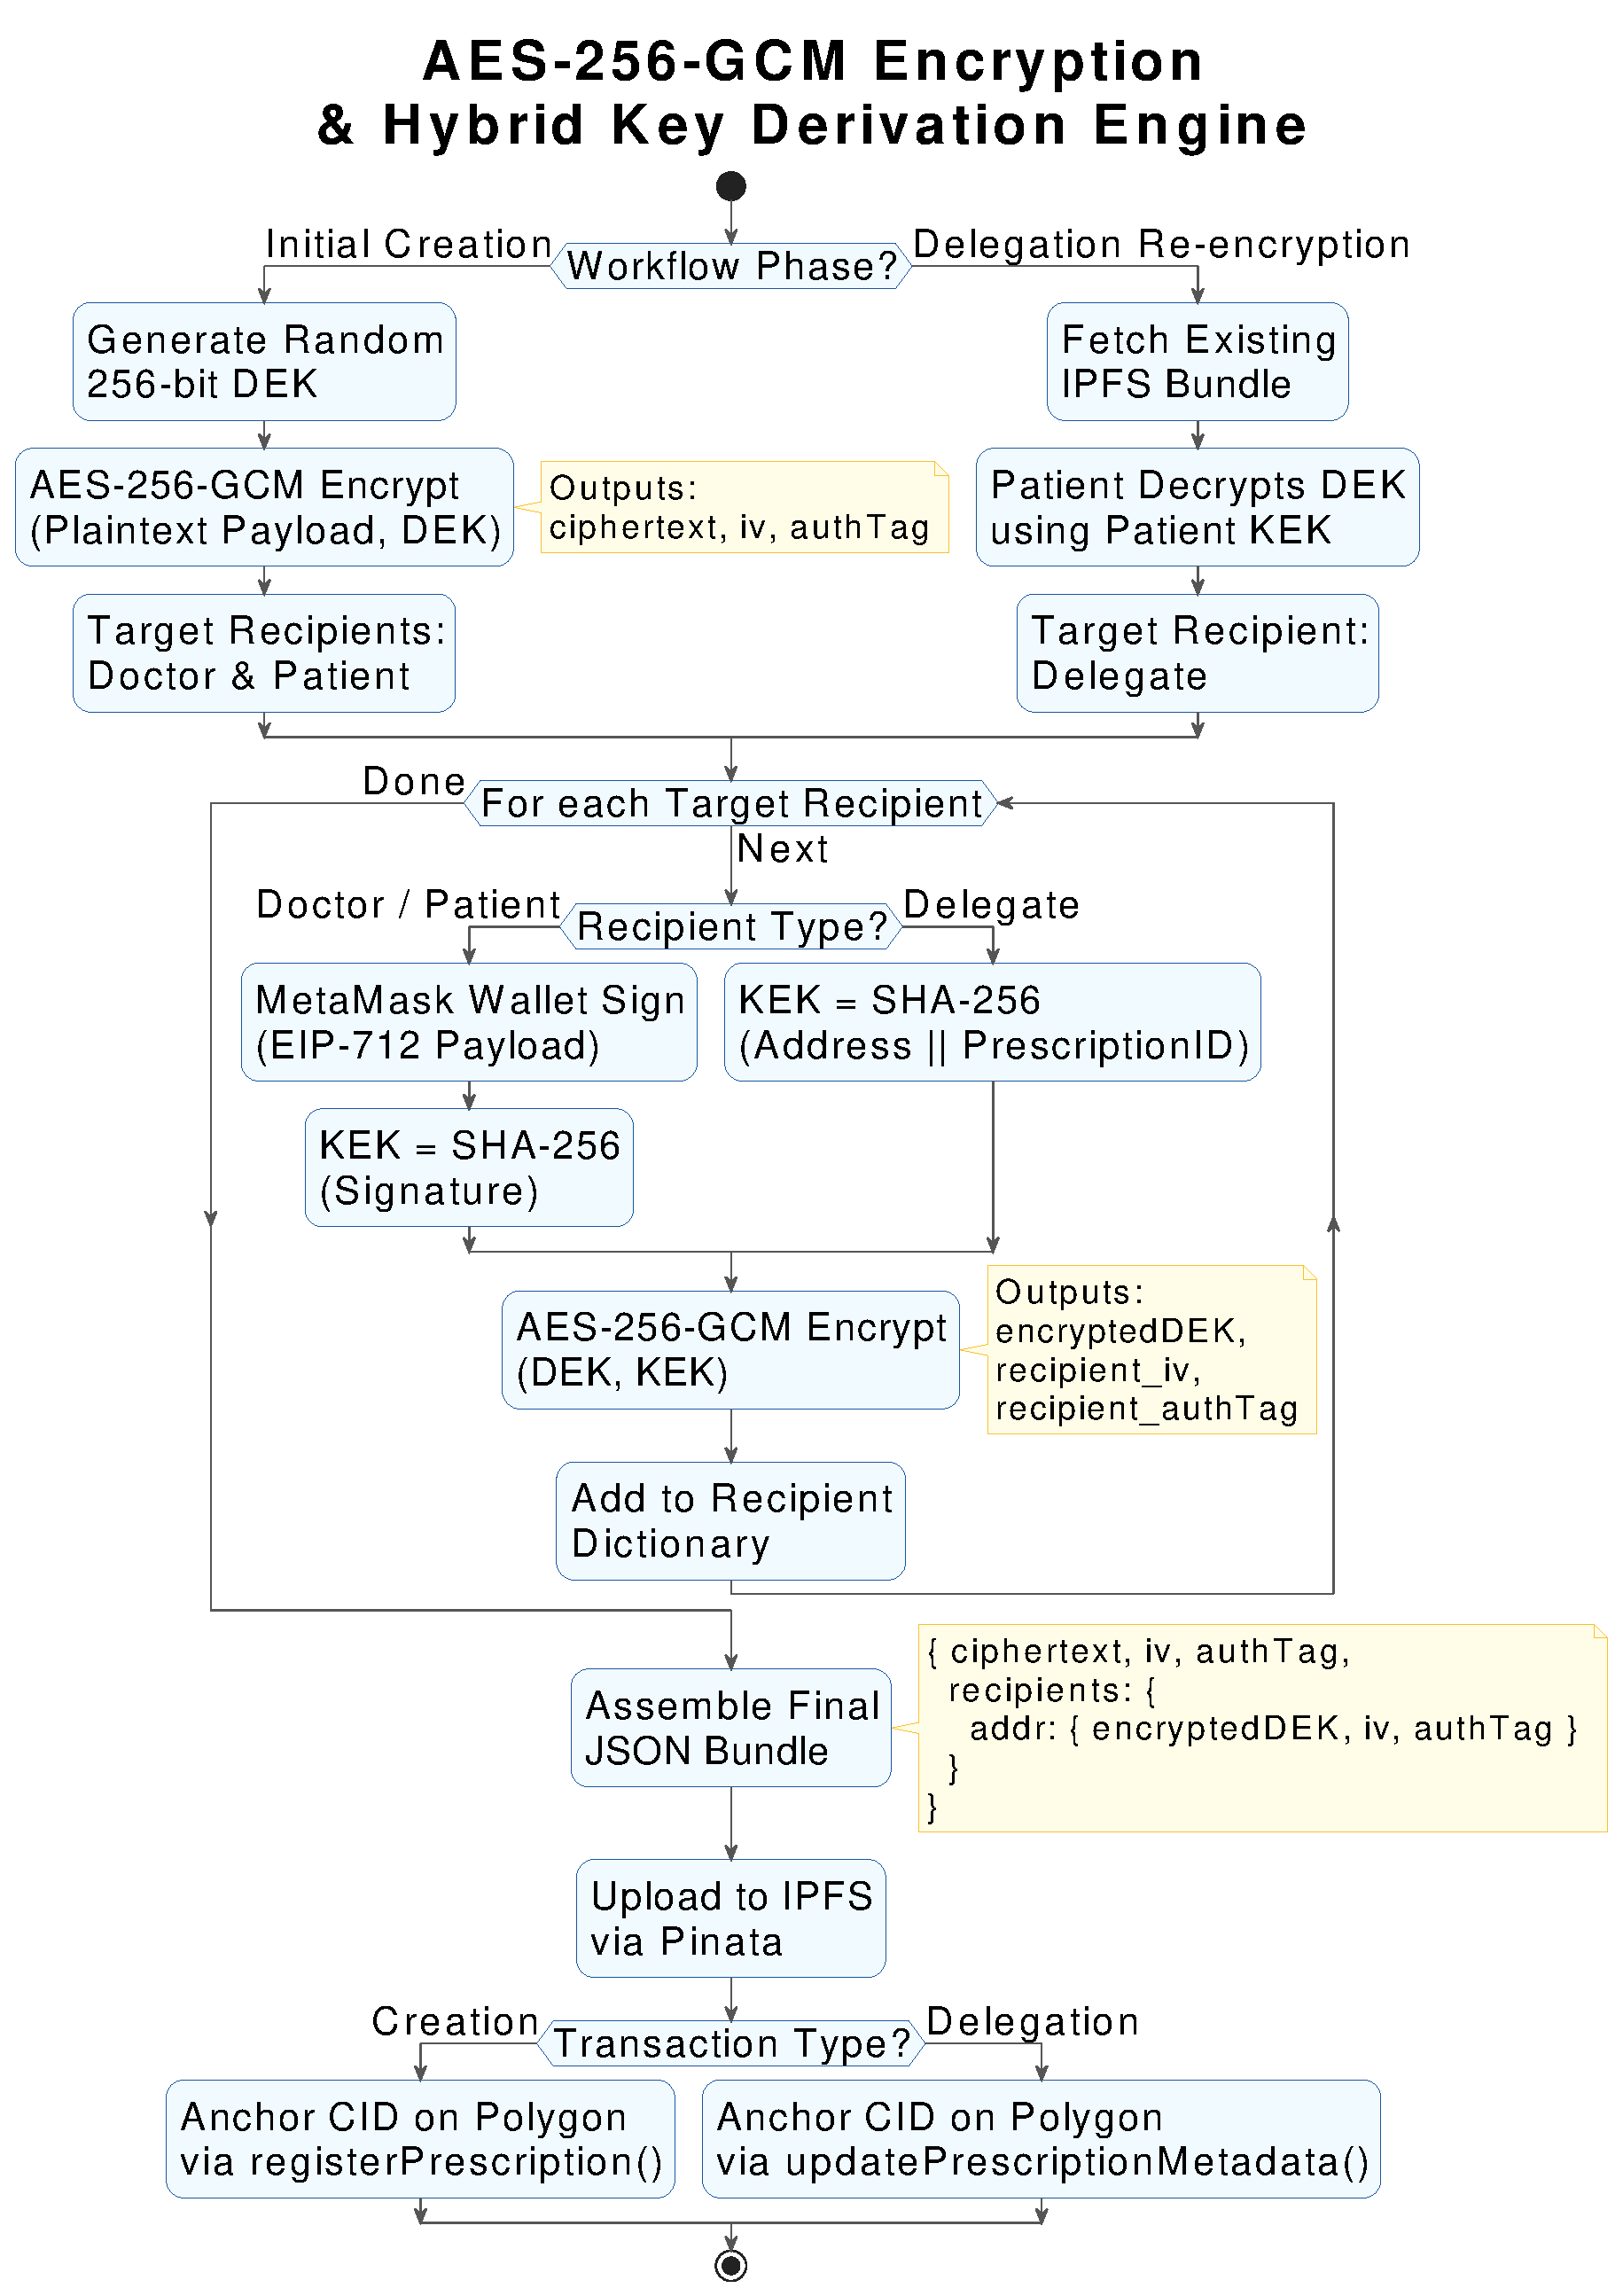
\includegraphics[width=\linewidth, height=0.75\textheight, keepaspectratio]{endToEnd_encryption.pdf}
\end{center}
\end{column}

\end{columns}
\end{frame}

\begin{frame}{Workflow Part 1: Draft \& Patient Review}
\begin{figure}
\centering
% Forces the image to maximize available space without overflowing
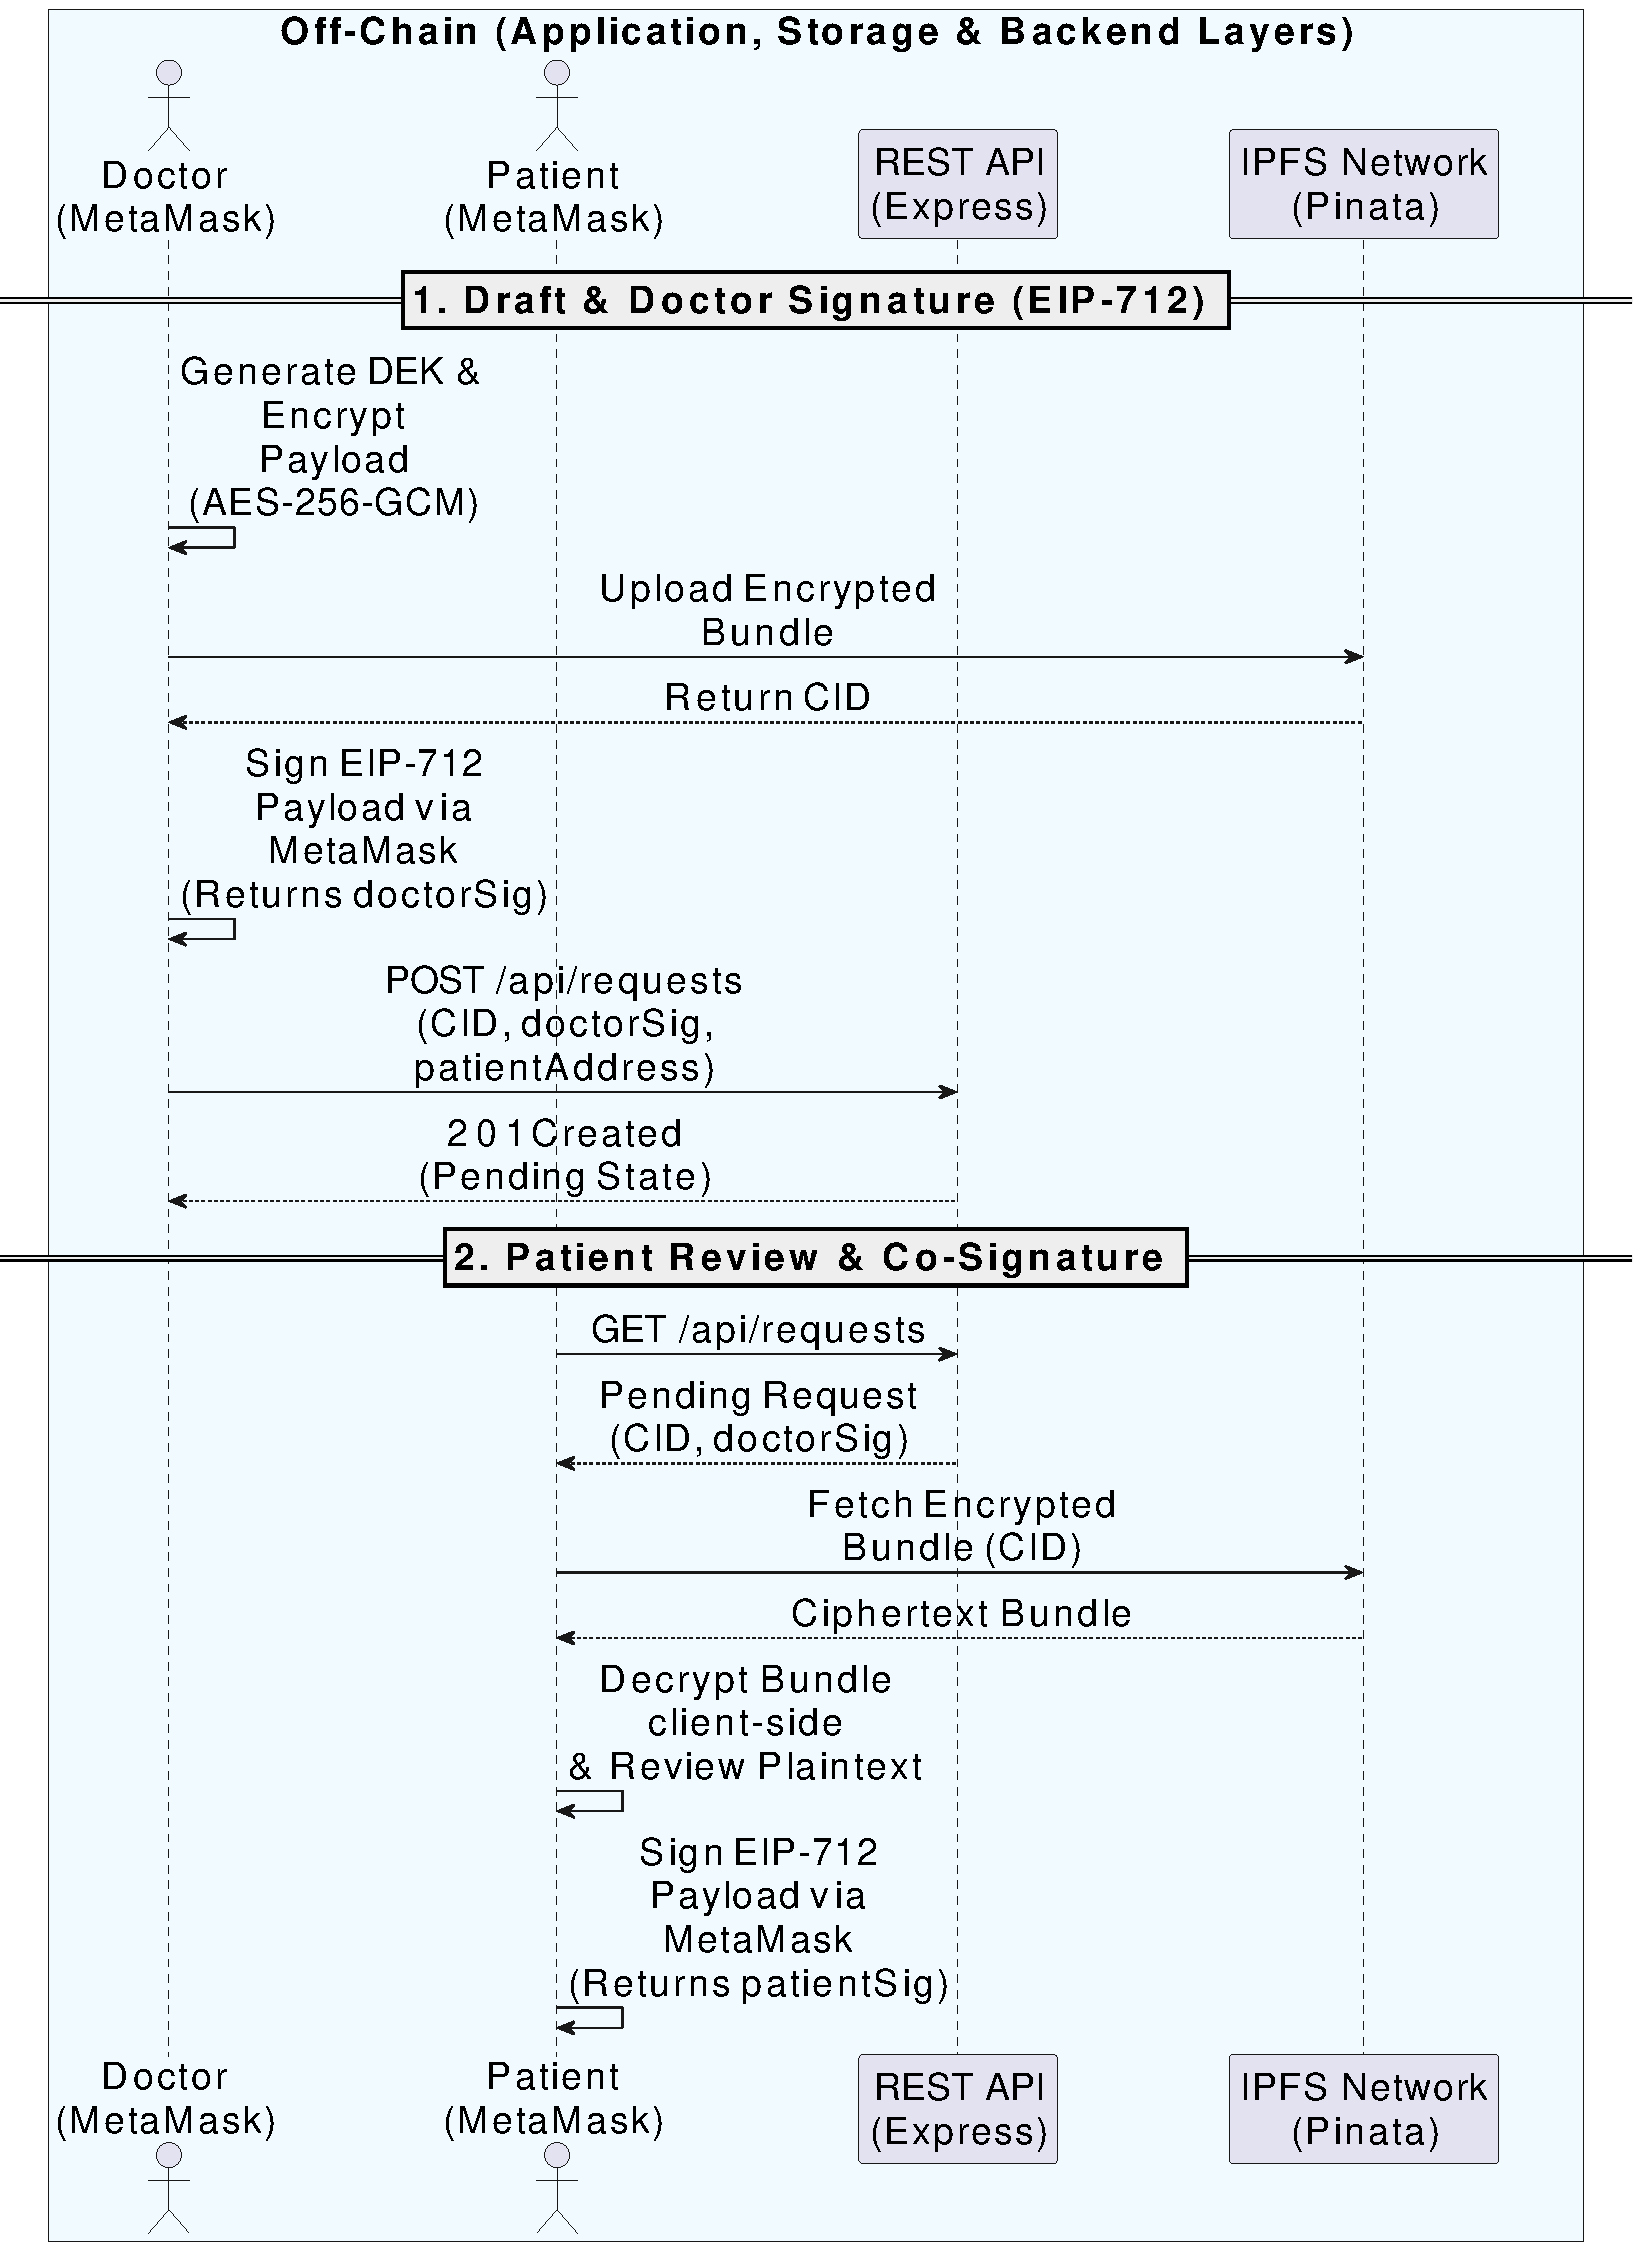
\includegraphics[width=1.0\textwidth, height=0.65\textheight, keepaspectratio]{sequenceDiagram_part1.pdf}
\end{figure}

\vspace{0.2cm}
\small
\begin{itemize}
  \item Pending approval is maintained off-chain in the request queue.
  \item The patient decrypts and reviews the full plaintext locally before signing.
\end{itemize}
\end{frame}

\begin{frame}{Workflow Part 2: On-Chain Commitment}

\vspace{-0.5cm} % Pulls the entire content up to prevent bottom clipping
\begin{center}
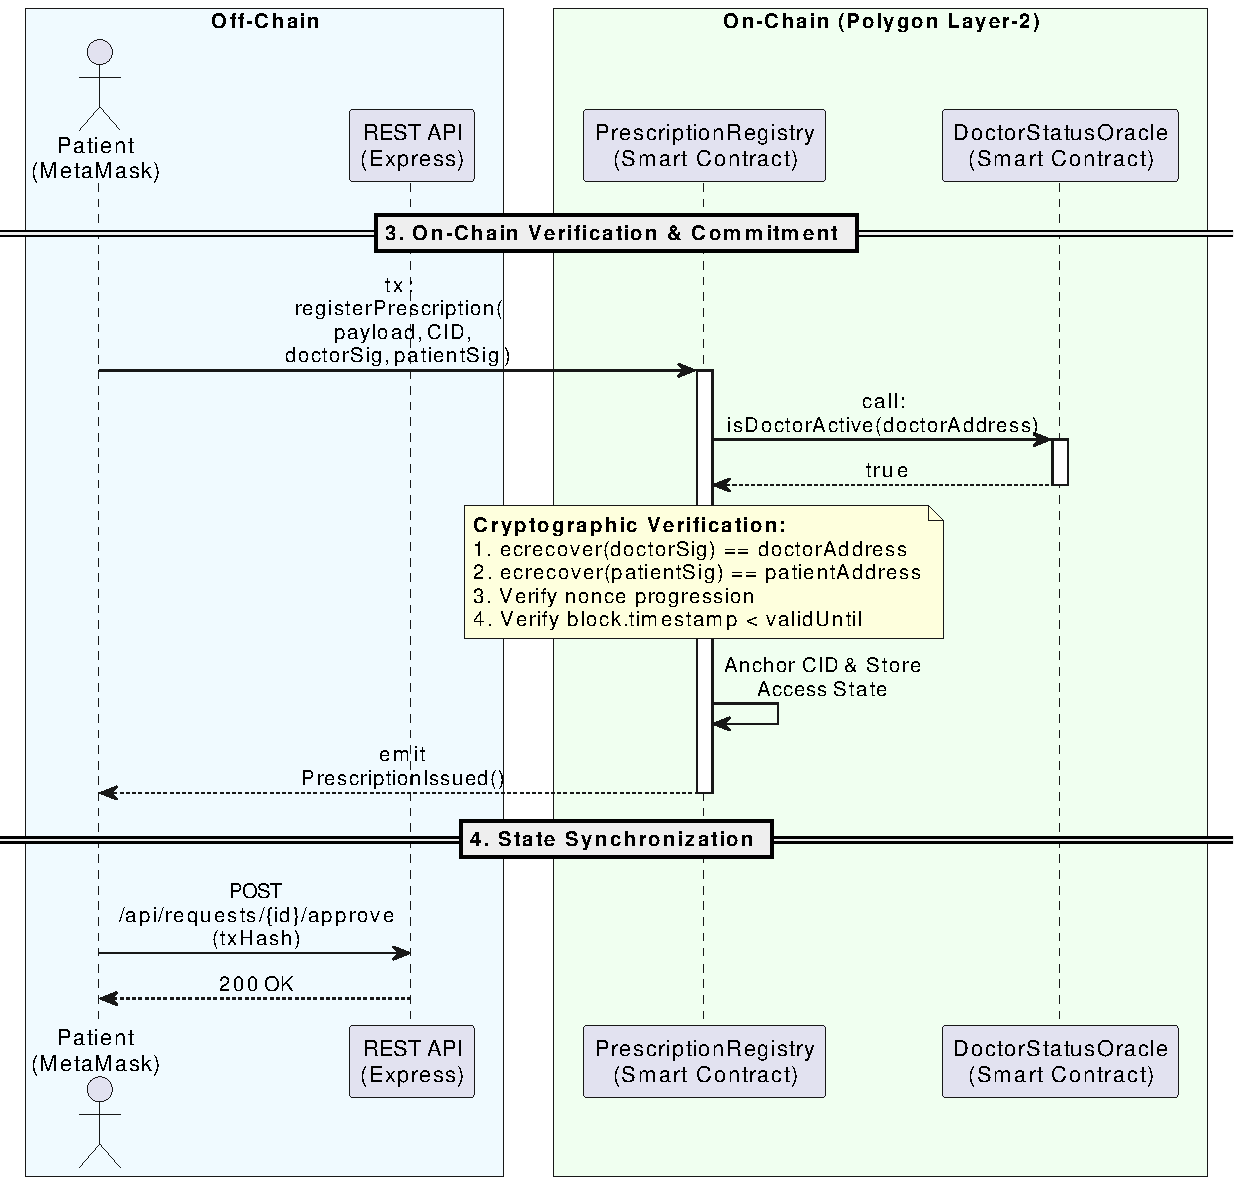
\includegraphics[height=0.6\textheight, keepaspectratio]{sequenceDiagram_part2.pdf}
\end{center}

\vspace{-0.1cm}
\footnotesize % Using a smaller font size for the explanatory text
\begin{itemize}
  \setlength{\itemsep}{0pt} % Removes vertical gaps between bullets
  \item Final publication occurs only when the patient signs and submits \texttt{registerPrescription()}.
  \item The contract verifies both signatures, nonces, and the doctor's oracle status.
\end{itemize}
\end{frame}
\begin{frame}{Implementation Summary}
\small
\begin{columns}[T]
\begin{column}{0.49\textwidth}
\textbf{Blockchain layer}
\begin{itemize}
  \item \texttt{PrescriptionRegistry}
  \item \texttt{DoctorStatusOracle}
  \item EIP-712 signature verification
  \item patient delegation and metadata update
\end{itemize}

\textbf{Application layer}
\begin{itemize}
  \item React + Vite + Wagmi + MetaMask
  \item role-specific doctor, patient, delegate, admin views
\end{itemize}
\end{column}
\begin{column}{0.49\textwidth}
\textbf{Backend and storage}
\begin{itemize}
  \item Node.js / Express request API
  \item Pinata orchestration for IPFS bundles
  \item request queue and metadata lookup
\end{itemize}

\textbf{Security mechanisms}
\begin{itemize}
  \item AES-256-GCM encrypted bundles
  \item nonce and expiry checks
  \item on-chain view authorization
\end{itemize}
\end{column}
\end{columns}
\end{frame}

\begin{frame}{Implementation and Demonstration Plan}
\small
\begin{enumerate}
  \item Admin whitelists a doctor in \texttt{DoctorStatusOracle}.
  \item Doctor creates a prescription request and signs the EIP-712 payload.
  \item Patient reviews the encrypted request, signs approval, and publishes it on-chain.
  \item System shows the anchored record with \texttt{prescriptionId} and \texttt{metadataURI}.
  \item Patient grants delegate access; the encrypted bundle is refreshed for the new recipient.
\end{enumerate}

\vspace{0.2cm}
\textbf{Presentation demo assets to show}
\begin{itemize}
  \item short prototype recording of the doctor-to-patient flow
  \item blockchain immutability simulation recording
  \item one results slide using generated metrics and benchmark outputs
\end{itemize}
\end{frame}


\begin{frame}{Why Blockchain Is Tamper-Evident}
\footnotesize
\begin{gather*}
\mathtt{dataHash} = H(\mathtt{encryptedBundle}) \\
\mathtt{blockHash} = H(\mathtt{index} \| \mathtt{timestamp} \| \mathtt{previousHash} \| \mathtt{dataHash} \| \mathtt{metadataURI})
\end{gather*}

\begin{center}
\IntegrityDiagram{0.68}
\end{center}

\vspace{-0.2cm}
\begin{itemize}
  \setlength{\itemsep}{0pt}
  \item If the encrypted record changes, the content hash changes.
  \item If the hash changes, the CID changes and the old on-chain anchor no longer matches.
  \item If a historical block changes, downstream \texttt{previousHash} references break.
\end{itemize}
\end{frame}

\begin{frame}{Measured Prototype Results}
\small
\begin{columns}[T]
\begin{column}{0.5\textwidth}
\begin{tabular}{@{}ll@{}}
\toprule
\textbf{Metric} & \textbf{Value} \\
\midrule
Draft creation & 13.38 s \\
Finalisation & 12.79 s \\
Delegate approval & 7.99 s \\
Pinata upload & 1.28 s \\
Encryption & 4.90 s \\
Decryption & 14 ms \\
API mean latency & 19.95 ms \\
register gas & 256,532 \\
delegate gas & 46,556 \\
Contract tests & 37 / 37 \\
\bottomrule
\end{tabular}
\end{column}

\begin{column}{0.48\textwidth}
\begin{tikzpicture}
\begin{axis}[
  ybar,
  width=\textwidth,
  height=0.58\textheight,
  ymin=0,
  ymax=16,
  ylabel={Time (s)},
  symbolic x coords={Draft,Finalize,Delegate,Pinata},
  xtick=data,
  xticklabel style={rotate=40, anchor=north east, font=\scriptsize},
  nodes near coords,
  nodes near coords style={font=\tiny},
  bar width=13pt,
  enlarge x limits=0.25,
  grid=major,
  grid style={dashed, gray!30}
]
\addplot[fill=blue!35, draw=blue!70!black] coordinates {
  (Draft,13.38) (Finalize,12.79) (Delegate,7.99) (Pinata,1.28)
};
\end{axis}
\end{tikzpicture}
\end{column}
\end{columns}

\vspace{0.1cm}
\footnotesize
\textbf{Inference:} end-to-end latency is dominated by user signing, encryption, and IPFS interaction rather than raw API overhead.
\end{frame}

\begin{frame}{Blockchain-Only Benchmark on Local Anvil}
\begin{columns}[T]
\begin{column}{0.58\textwidth}
\begin{tikzpicture}
\begin{axis}[
  width=\textwidth,
  height=0.54\textheight,
  xlabel={Transaction count},
  ylabel={Average latency (ms)},
  xmin=1.5, xmax=5.5,
  ymin=650, ymax=1200,
  grid=major,
  grid style={dashed, gray!30},
  legend pos=north west,
  legend style={font=\tiny}
]
\addplot[color=blue!70!black, mark=*] coordinates {(2,927.5) (5,969.8)};
\addlegendentry{register sequential}
\addplot[color=red!70!black, mark=square*] coordinates {(2,720.0) (5,1148.2)};
\addlegendentry{register burst}
\addplot[color=green!60!black, mark=triangle*] coordinates {(2,1127.5) (5,963.2)};
\addlegendentry{delegate sequential}
\addplot[color=orange!80!black, mark=diamond*] coordinates {(2,722.0) (5,1135.6)};
\addlegendentry{delegate burst}
\end{axis}
\end{tikzpicture}
\end{column}
\begin{column}{0.40\textwidth}
\small
\textbf{Representative verification run}
\begin{itemize}
  \item single-node Anvil
  \item sequential and burst modes
  \item real contract transactions
\end{itemize}

\textbf{Meaning}
\begin{itemize}
  \item isolates blockchain behaviour from frontend and IPFS
  \item burst mode is the relevant stress case
  \item this is not a multi-validator scalability result
\end{itemize}
\end{column}
\end{columns}
\end{frame}

% --- REPLACE YOUR WORKLOAD PROJECTION SLIDE WITH THIS ---
\begin{frame}{Workload Projection Based on Measured Averages}
\small
\[
\mathtt{estimatedTotalGas} \approx
\begin{aligned}
&(\mathtt{prescriptionCount} \times \overline{\mathtt{registerGas}})\\
&+ (\mathtt{delegateCount} \times \overline{\mathtt{delegateGas}})
\end{aligned}
\]

\begin{center}
\begin{tikzpicture}
\begin{axis}[
  width=0.9\textwidth,
  height=0.42\textheight, % <--- STRICT HEIGHT LIMIT TO PREVENT TOP CUT-OFF
  xlabel={Prescription count},
  ylabel={Estimated gas units},
  xmin=0, xmax=520,
  ymin=0, ymax=160000000, % <--- INCREASED TO FIT THE 1.33 * 10^8 LABEL
  scaled y ticks=false,
  grid=major,
  grid style={dashed, gray!30},
  nodes near coords,
  nodes near coords style={font=\tiny, anchor=south} % <--- FLOATS TEXT ABOVE DOTS
]
\addplot[color=purple!75!black, mark=*] coordinates {
  (25,6646080) (100,26584320) (500,132921600)
};
\end{axis}
\end{tikzpicture}
\end{center}

\vspace{0.1cm}
\footnotesize
\textbf{Inference:} cumulative cost grows approximately linearly in the current projection because only compact metadata is anchored on-chain while the medical payload remains off-chain.
\end{frame}


\begin{frame}{Security and Correctness Evidence}
\begin{columns}[c]

\begin{column}{0.48\textwidth}
\footnotesize 
\begin{itemize}
  \setlength{\itemsep}{0.5ex} 
  \item \textbf{Contract correctness:} 37/37 Foundry tests passed.
  \item \textbf{Role enforcement:} inactive doctors/invalid signatures rejected.
  \item \textbf{Replay resistance:} nonce progression breaks replayed signatures.
  \item \textbf{View protection:} unauthorized viewers receive denial on fetch.
  \item \textbf{Tamper evidence:} CID mismatch demonstrated by simulation.
\end{itemize}

\vspace{0.15cm}
\textbf{Four evidence types:}
\begin{itemize}
  \setlength{\itemsep}{0.5ex} 
  \item implementation correctness
  \item measured latency and gas
  \item blockchain-layer benchmark
  \item simulation-based scaling
\end{itemize}
\end{column}

\begin{column}{0.52\textwidth}
\begin{figure}
\centering
\resizebox{\linewidth}{!}{
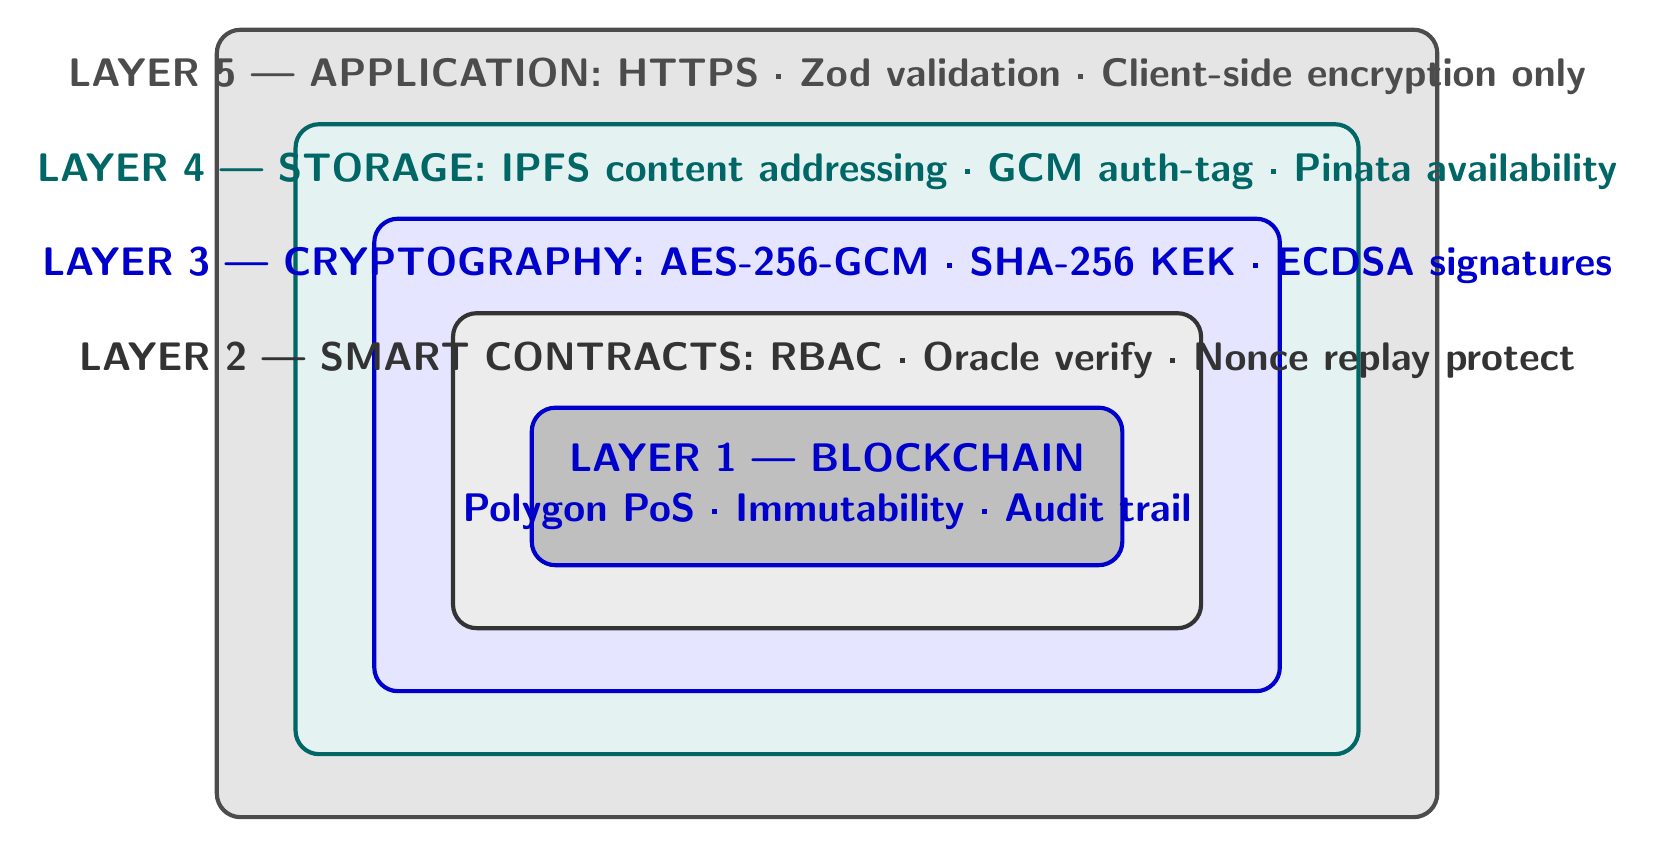
\begin{tikzpicture}[
  secring/.style={draw=#1, line width=1.5pt, rounded corners=3mm}
]

% Layer 5
\node[secring=black!70, fill=gray!20, minimum width=15.5cm, minimum height=10.0cm] (L5) at (0,0) {};
\node[font=\Large\bfseries, text=black!70] at (0, 4.4)
  {LAYER 5 --- APPLICATION: HTTPS · Zod validation · Client-side encryption only};

% Layer 4
\node[secring=teal!80!black, fill=teal!10, minimum width=13.5cm, minimum height=8.0cm] (L4) at (0,-0.2) {};
\node[font=\Large\bfseries, text=teal!80!black] at (0, 3.2)
  {LAYER 4 --- STORAGE: IPFS content addressing · GCM auth-tag · Pinata availability};

% Layer 3
\node[secring=blue!80!black, fill=blue!10, minimum width=11.5cm, minimum height=6.0cm] (L3) at (0,-0.4) {};
\node[font=\Large\bfseries, text=blue!80!black] at (0, 2.0)
  {LAYER 3 --- CRYPTOGRAPHY: AES-256-GCM · SHA-256 KEK · ECDSA signatures};

% Layer 2
\node[secring=black!80, fill=gray!15, minimum width=9.5cm, minimum height=4.0cm] (L2) at (0,-0.6) {};
\node[font=\Large\bfseries, text=black!80] at (0, 0.8)
  {LAYER 2 --- SMART CONTRACTS: RBAC · Oracle verify · Nonce replay protect};

% Layer 1
\node[secring=blue!80!black, fill=gray!50, minimum width=7.5cm, minimum height=2.0cm] (L1) at (0,-0.8) {};
\node[font=\Large\bfseries, text=blue!80!black, align=center] at (0,-0.8)
  {LAYER 1 --- BLOCKCHAIN\\Polygon PoS · Immutability · Audit trail};



\end{tikzpicture}
}
\caption{Five-layer security architecture}
\end{figure}
\end{column}

\end{columns}
\end{frame}


\begin{frame}{Applications of the Proposed Work}
\small
\begin{itemize}
  \item \textbf{Inter-hospital prescription portability:} a patient can carry anchored prescriptions across providers.
  \item \textbf{Telemedicine:} remote doctor issuance with patient co-approval before final publication.
  \item \textbf{Specialist referrals:} patient can delegate selective access to a specialist or laboratory.
  \item \textbf{Auditable health data exchange:} publication and delegation decisions remain on-chain and traceable.
  \item \textbf{Foundation for broader EHR workflows:} the same pattern can later extend to lab reports, referrals, and clinical notes.
\end{itemize}
\end{frame}


\begin{frame}{Limitations and Practical Constraints}
\small
\begin{itemize}
  \item current validation is primarily on a local Anvil chain, not a real multi-validator blockchain network
  \item plaintext-compatible API paths still exist, so the backend is best described as encrypted-first, not strictly zero-knowledge
  \item compliance with HIPAA or GDPR is not claimed; production deployment would need legal, operational, and infrastructure validation
  \item there is no emergency access override and no full hospital information system integration yet
  \item the request store is still file-based and should move to a real database for production-style usage
\end{itemize}
\end{frame}

\begin{frame}{Conclusion}
\small
\begin{itemize}
  \item \textbf{Definition and scope:} we implemented a blockchain-based prescription record prototype with patient-approved publication and auditable access control.
  \item \textbf{Literature position:} prior work often shows access control, performance, or load evidence, but not this exact combination of workflow and evaluation.
  \item \textbf{Architecture and implementation:} the proposed system combines browser-side encryption, IPFS storage, and smart-contract anchoring through \texttt{PrescriptionRegistry} and \texttt{DoctorStatusOracle}.
  \item \textbf{Applications:} the design is directly relevant to prescription portability, telemedicine, specialist referrals, and auditable health data exchange.
  \item \textbf{Key result:} the prototype is functionally correct, measurable, and explainable, while the evaluation package shows both what has been achieved and what remains future work.
\end{itemize}
\end{frame}

\begin{frame}{Demo Links and Resources}
\small
\begin{columns}[T]
\begin{column}{0.48\textwidth}
\textbf{Prototype demos}
\begin{itemize}
  \item Basic flow demo: \texttt{https://youtu.be/KZ4PxqNWKyU}
  \item Oracle / encryption / EIP-712 demo: \texttt{https://youtu.be/FmP9Ht6ha40}
  \item Integrity demo: \texttt{https://youtu.be/Q1TVN60fmX8}
\end{itemize}
\end{column}
\begin{column}{0.48\textwidth}
\textbf{Project resource}
\begin{itemize}
  \item GitHub repository: \texttt{https://github.com/U-Shashank/btp}
\end{itemize}

\vspace{0.2cm}
\end{column}
\end{columns}
\end{frame}

\begin{frame}{Demo Screenshots I}
\begin{center}

\begin{tikzpicture}[font=\sffamily]
  \node[draw=gray!60, rounded corners=4pt, minimum width=0.95\textwidth, minimum height=7.5cm, inner sep=6pt, fill=gray!5] at (0,0) {
    \IfFileExists{demo1.jpg}{
      \includegraphics[width=0.92\textwidth,height=7cm,keepaspectratio]{demo1.jpg}
    }{
      \fbox{\rule{0pt}{7cm}\rule{0.92\textwidth}{0pt}}
    }
  };
\end{tikzpicture}
\end{center}
\end{frame}

\begin{frame}{Demo Screenshots II}
\begin{center}

\begin{tikzpicture}[font=\sffamily]
  \node[draw=gray!60, rounded corners=4pt, minimum width=0.95\textwidth, minimum height=7.5cm, inner sep=6pt, fill=gray!5] at (0,0) {
    \IfFileExists{demo5.jpg}{
      \includegraphics[width=0.92\textwidth,height=7cm,keepaspectratio]{demo5.jpg}
    }{
      \fbox{\rule{0pt}{7cm}\rule{0.92\textwidth}{0pt}}
    }
  };
\end{tikzpicture}
\end{center}
\end{frame}

\begin{frame}{Demo Screenshots III}
\begin{center}

\begin{tikzpicture}[font=\sffamily]
  \node[draw=gray!60, rounded corners=4pt, minimum width=0.95\textwidth, minimum height=7.5cm, inner sep=6pt, fill=gray!5] at (0,0) {
    \IfFileExists{demo3.jpg}{
      \includegraphics[width=0.92\textwidth,height=7cm,keepaspectratio]{demo3.jpg}
    }{
      \fbox{\rule{0pt}{7cm}\rule{0.92\textwidth}{0pt}}
    }
  };
\end{tikzpicture}
\end{center}
\end{frame}

\begin{frame}{Demo Screenshots IV}
\begin{center}

\begin{tikzpicture}[font=\sffamily]
  \node[draw=gray!60, rounded corners=4pt, minimum width=0.95\textwidth, minimum height=7.5cm, inner sep=6pt, fill=gray!5] at (0,0) {
    \IfFileExists{demo4.jpg}{
      \includegraphics[width=0.92\textwidth,height=7cm,keepaspectratio]{demo4.jpg}
    }{
      \fbox{\rule{0pt}{7cm}\rule{0.92\textwidth}{0pt}}
    }
  };
\end{tikzpicture}
\end{center}
\end{frame}

\begin{frame}
\vfill
\begin{center}
    
\begin{tikzpicture}[font=\sffamily]
        \node[
            rectangle, 
            rounded corners=12pt, 
            draw=blue!60, 
            top color=blue!5, 
            bottom color=white,
            thick,
            minimum width=0.85\textwidth,
            minimum height=4.5cm,
            drop shadow={opacity=0.15, shadow xshift=2pt, shadow yshift=-2pt}
        ] (thanks) {
            \begin{tabular}{c}
                {\Huge \textbf{\textcolor{blue!80!black}{Thank You!}}} \\[0.8cm]
                {\Large \textbf{Questions \& Discussion}} \\[0.4cm]
                \textcolor{gray!80!black}{\small We welcome your feedback and queries.}
            \end{tabular}
        };
    \end{tikzpicture}
\end{center}
\vfill
\end{frame}

\end{document}
